% $Id: template.tex 11 2007-04-03 22:25:53Z jpeltier $

\documentclass{vgtc}                          % final (conference style)
%\documentclass[review]{vgtc}                 % review
%\documentclass[widereview]{vgtc}             % wide-spaced review
%\documentclass[preprint]{vgtc}               % preprint
%\documentclass[electronic]{vgtc}             % electronic version

%% Uncomment one of the lines above depending on where your paper is
%% in the conference process. ``review'' and ``widereview'' are for review
%% submission, ``preprint'' is for pre-publication, and the final version
%% doesn't use a specific qualifier. Further, ``electronic'' includes
%% hyperreferences for more convenient online viewing.

%% Please use one of the ``review'' options in combination with the
%% assigned online id (see below) ONLY if your paper uses a double blind
%% review process. Some conferences, like IEEE Vis and InfoVis, have NOT
%% in the past.

%% Figures should be in CMYK or Grey scale format, otherwise, colour 
%% shifting may occur during the printing process.

%% These three lines bring in essential packages: ``mathptmx'' for Type 1 
%% typefaces, ``graphicx'' for inclusion of EPS figures. and ``times''
%% for proper handling of the times font family.

\usepackage{mathptmx}
\usepackage{graphicx}
\usepackage{times}
\usepackage{mathtools}
\usepackage{graphicx}
%% We encourage the use of mathptmx for consistent usage of times font
%% throughout the proceedings. However, if you encounter conflicts
%% with other math-related packages, you may want to disable it.

%% If you are submitting a paper to a conference for review with a double
%% blind reviewing process, please replace the value ``0'' below with your
%% OnlineID. Otherwise, you may safely leave it at ``0''.
\onlineid{0}

%% declare the category of your paper, only shown in review mode
\vgtccategory{Research}

%% allow for this line if you want the electronic option to work properly
\vgtcinsertpkg

%% In preprint mode you may define your own headline.
%\preprinttext{To appear in an IEEE VGTC sponsored conference.}

%% Paper title.

\title{NvPipe: A Lightweight H264-based Hardware Accelerated Image Compression Library}

%% This is how authors are specified in the conference style

%% Author and Affiliation (single author).
%%\author{Roy G. Biv\thanks{e-mail: roy.g.biv@aol.com}}
%%\affiliation{\scriptsize Allied Widgets Research}

%% Author and Affiliation (multiple authors with single affiliations).
%%\author{Roy G. Biv\thanks{e-mail: roy.g.biv@aol.com} %
%%\and Ed Grimley\thanks{e-mail:ed.grimley@aol.com} %
%%\and Martha Stewart\thanks{e-mail:martha.stewart@marthastewart.com}}
%%\affiliation{\scriptsize Martha Stewart Enterprises \\ Microsoft Research}

%% Author and Affiliation (multiple authors with multiple affiliations)
%%\author{Roy G. Biv\thanks{e-mail: roy.g.biv@aol.com}\\ %
%%        \scriptsize Starbucks Research %
%%\and Ed Grimley\thanks{e-mail:ed.grimley@aol.com}\\ %
%%     \scriptsize Grimley Widgets, Inc. %
%%\and Martha Stewart\thanks{e-mail:martha.stewart@marthastewart.com}\\ %
%%     \parbox{1.4in}{\scriptsize \centering Martha Stewart Enterprises \\ Microsoft Research}}
\author{Jie Jiang \thanks{e-mail: jjiang24@uic.edu}\\ %
        \scriptsize University of Illinois at Chicago %
\and Tom Fogal\thanks{e-mail:tfogal@nvidia.com}\\ %
     \scriptsize NVIDIA %
\and Cliff Woolley\thanks{e-mail:jwoolley@nvidia.com}\\ %
     \scriptsize NVIDIA}


%% A teaser figure can be included as follows, but is not recommended since
%% the space is now taken up by a full width abstract.
%\teaser{
%  \includegraphics[width=1.5in]{sample.eps}
%  \caption{Lookit! Lookit!}
%}

%% Abstract section.
\abstract{
NvPipe is a lightweight image compression library that utilizes H.264 standard and NVIDIA hardware accelerated API. Our benchmark results and experiments with ParaView integration shows superior compression ratio gain and performance of NvPipe over ParaView built-in compressors. It reveals great potential of its application in image streaming over network with limited bandwidth.
} % end of abstract

%% ACM Computing Classification System (CCS). 
%% See <http://www.acm.org/class/1998/> for details.
%% The ``\CCScat'' command takes four arguments.

%\CCScatlist{ 
%  \CCScat{K.6.1}{Management of Computing and Information Systems}%
%{Project and People Management}{Life Cycle};
%  \CCScat{K.7.m}{The Computing Profession}{Miscellaneous}{Ethics}
%}

%% Copyright space is enabled by default as required by guidelines.
%% It is disabled by the 'review' option or via the following command:
% \nocopyrightspace

%%%%%%%%%%%%%%%%%%%%%%%%%%%%%%%%%%%%%%%%%%%%%%%%%%%%%%%%%%%%%%%%
%%%%%%%%%%%%%%%%%%%%%% START OF THE PAPER %%%%%%%%%%%%%%%%%%%%%%
%%%%%%%%%%%%%%%%%%%%%%%%%%%%%%%%%%%%%%%%%%%%%%%%%%%%%%%%%%%%%%%%%

\begin{document}

%% The ``\maketitle'' command must be the first command after the
%% ``\begin{document}'' command. It prepares and prints the title block.

%% the only exception to this rule is the \firstsection command
\firstsection{Introduction}

\maketitle

Image compression is commonly used in distributed visualization systems to overcome limitations of available bandwidth. Conventional image compression approach focuses on removing redundant information within each image without necessarily utilizing the inter-frame coherency.

H.264 is a block-oriented motion-compensation-based video compression standard. It provides high compression capability at the cost of significant computational expenses. NVIDIA provides hardware accelerated H.264 encoder since Kepler archetecture. It enables real-time encoding with minimum overhead through NVIDIA codec API and it has been integrated into multimedia framework FFmpeg. 

\section{Implementation}

NvPipe is built on top of FFmpeg to provide compatibility on systems with either CPU or accelerated GPU.

\subsection{Design}

NvPipe is implemented on top of FFmpeg to provide compatibility to both CPU-only and GPU-accelerated systems. It uses libx264 codec on CPU and NVIDIA codec on GPU. 

The principle of the interface design of NvPipe is simplicity. It expects the user with minimum knowledge about video encoding and requires little effort to set up.

Encoding and decoding with NvPipe is implemented in a synchronous manner without frame latency. Each input frame/packet guarantees a corresponding output packet/frame. Both input and output buffer are allocated and provided by user on host memory.

\subsection{Performance}

The performance of the compression library is measure by 3 factors which are compression ratio, computational efficiency and image quality preservation.

\subsubsection{Compression Ratio}

%put the reference here: http://www.adobe.com/content/dam/Adobe/en/devnet/video/articles/h264_primer/h264_primer.pdf
Average bitrate parameter for encoder determines the bandwidth of encoded data, i.e. compression ratio. A guideline for bitrate setting is through formula:

\begin{equation}
\label{formula:bitrate}
 bitrate = resolution * \text{ fps} * f_m * 0.07
\end{equation}

Where \(f_m\) is the motion factor that defines the estimated motion of the video with value of [1...4]. While 1 stands for low motion and 4 for high motion.

Assuming we are given 8bit RGB image. Each pixel contains 3 channel of image data. The compression ratio could be defined by dividing the bitrate to the total generated image data per second.

\begin{equation}
\label{formula:compress_ratio}
 r = \frac{ \text{ bitrate}}{ \text{ resolution} * \text{ fps} * f_m * 3 * 8} = 0.07/3/8 = 0.29\%
\end{equation}

\subsubsection{Computational Expenses}
% image conversion and API call

Each image compression or decompression call to NvPipe consists of format conversion and encoding or decoding API calls. Computational complexity for both tasks are linear to the totally number of pixels of the input or output image. So we could expect the overall complexity of our compression and decompression call remains linear to the image size.

\subsubsection{Image Quality}

NvPipe could possibly deteriorate image quality at both stage. The image format conversion applies chroma subsampling that could introduce error on sharp edges. Meanwhile H.264 is also lossy compression. \ref{figure:quality} shows the image recovery quality. For normal visualization images using recommended encoding bitrate only introduces negligible difference. The Structural Similarity (SSIM) between two image on the left is 0.9986. Even after siginificant white noise being added to the original image we start to have perceivable quality drops. The SSIM between two images on the right is 0.7861.

\begin{figure}[htb]
  \label{figure:quality}
  \centering
  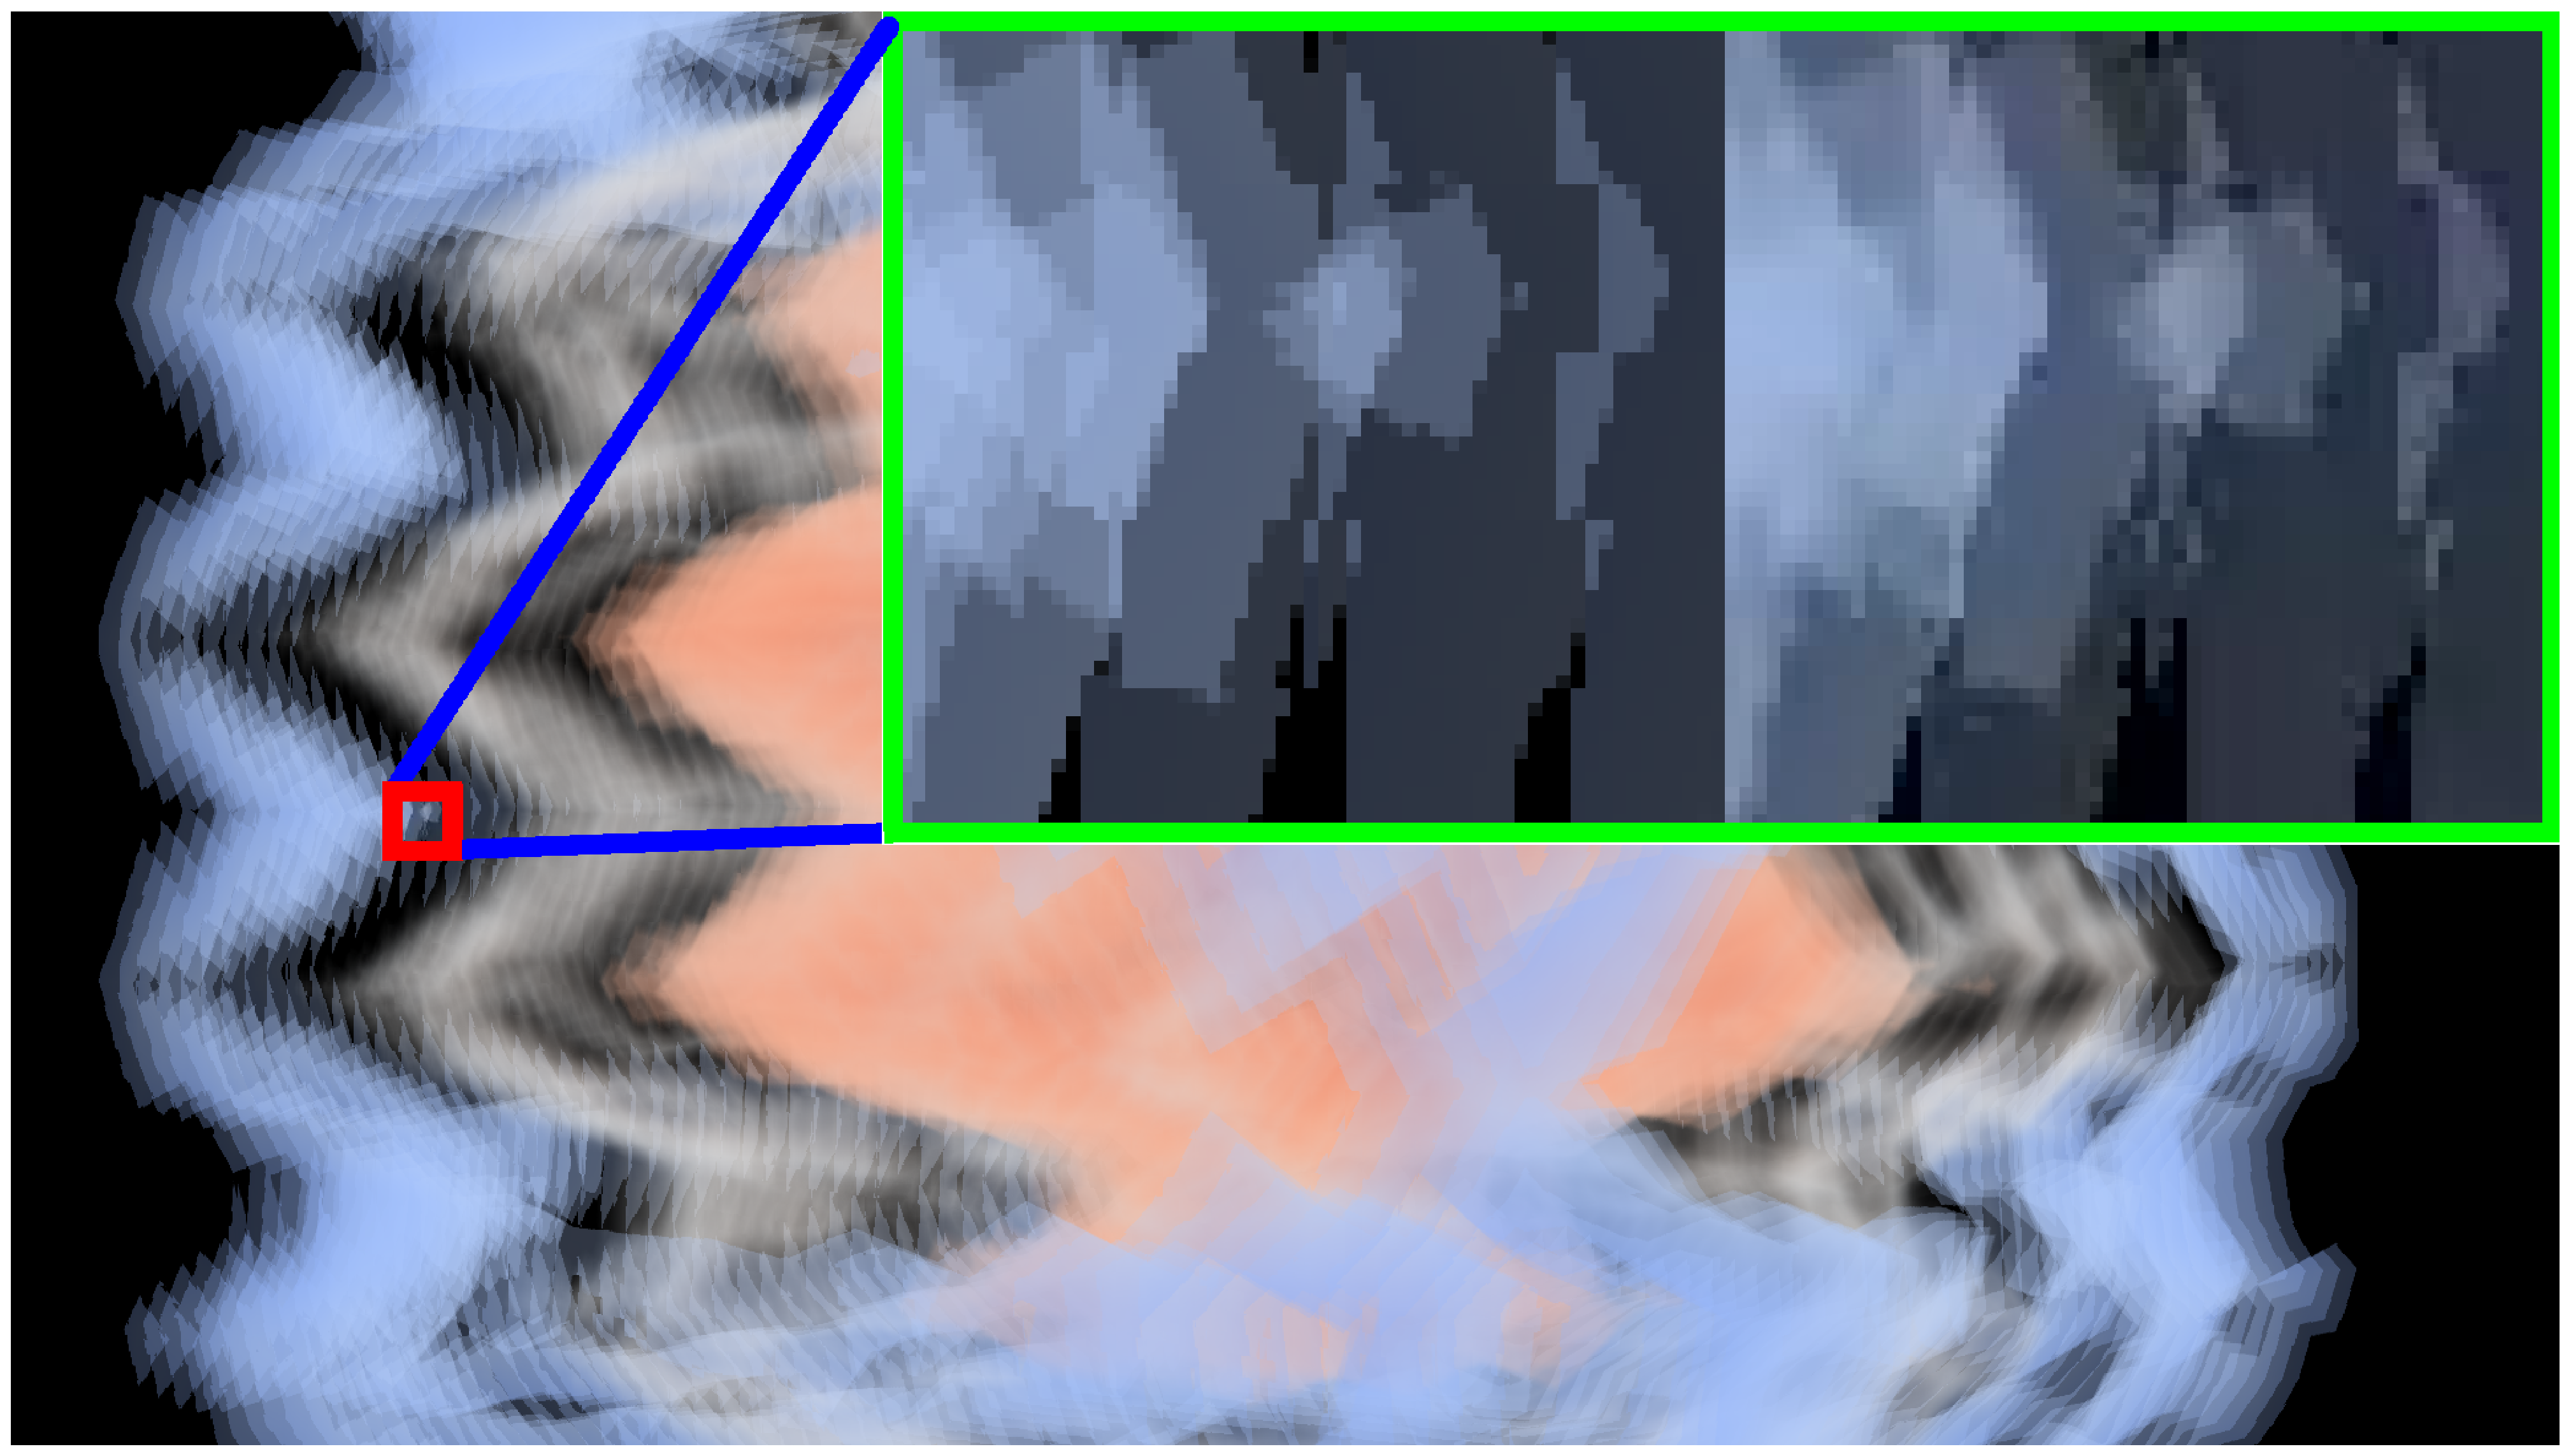
\includegraphics[width=3in]{quality.eps}
  \caption{Image quality reservation: images on top are the original while the bottom ones are the recovered. The right column uses the left column image with artificially added white noise.}
\end{figure}


\section{Experiment}

Our experiment setup contains two parts. In part one we benchmark the performance of our library given different resolutions and bitrates. In part two we implement vtkNvpipeCompressor to integrate NvPipe into Paraview. We create a distribute visualization use case and compared the performance of NvPipe with ParaView\'s native built-in compressor.

\subsection{Experiment Setup}
% library benchmark
Our experiment runs on a linux machines powered by NVIDIA GFORCE GTX 1080 (PASCAL) graphics card.

\subsubsection{NvPipe Benchmark}

To verify the linear computational complexity property, we have 4 experiment groups set up as \ref{table:experiment_setup}. For each resolution we also have 3 cases with various bitrate. The medium bitrate is the bitrate calculated using \ref{formula:bitrate} with \(f_m = 1\). While the low bitrate and high bitrate are calculated using a factor of 0.5 and 2 respectively. Each session runs 300 circles of consecutive motion image.

\begin{table}
  \caption{Computational Scalability Experiment measuring encoding and decoding time with RGB images}
  \label{table:experiment_setup}
  \scriptsize
  \begin{center}
    \begin{tabular}{cccc}
      Format & Resolution & Number of pixels & Medium Bitrate (mbps)\\
    \hline
      XGA &  1024x768 & 786432 & 1.651\\
      720P & 1280x720 & 921600 & 1.935\\
      1080P & 1920x1080 & 2073600 & 4.355\\
      4k & 4096x2160 & 8847360 & 18.579
    \end{tabular}
  \end{center}
\end{table}

\subsubsection{ParaView Integration}

In this distributed visualization ParaView server use NvPipe to compress rendered image before sending it to the client GUI. Then it decompress the received packet to restore the image. Both server and client are launched on the same machine and sharing resources.

For each execution, we visualize the wavelet dataset and rotate it to render 100 frames image. We compare NvPipe with 3 other libraries. Each native compressor use its optimal compression setting that yields maximum compression ratio. While NvPipe is set to use the default bitrate.

\subsection{Results}

\begin{figure}[htb]
  \label{figure:linear}
  \centering
  \includegraphics[width=2.0in]{linear.eps}
  \caption{X-axis is the number of pixels while Y-axis is the processing time in milliseconds}
\end{figure}

% insert the encoding/decoding time graph here (maybe we should re run it with stacked info)
From our experiment result \ref{figure:linear}, we verify that compression and decompression time stay linear to the size of image and remains independent of bitrate usage.

% discuss the bandwidth reduction ( compare other paraview compressor )
NvPipe demonstrates significant advantage over all ParaView built-in image compressor for bandwidth reduction. \ref{table:compression_ratio} shows that NvPipe achieves an average compression ratio of 0.32\%. While the next best compressor Zlib could only achieve 4.87\% compression ratio. From \ref{figure:compressRatio} and the standard deviation from \ref{table:compression_ratio} we observe that NvPipe provides more stable output rate. While images processed by other compressors tends to have varying sizes between frames.

NvPipe exhibits competitive efficiency among other compressors in \ref{figure:time}. The average overall compression and decompression time is only 12.78ms. And the average encoding and decoding time for FFmpeg API call are 3.938ms and 3.029ms. They yield framerates of 254fps and 330fps respectively. Because of the overhead introduced through FFmpeg wrapper they are expected to be lower than 398fps/658fps released by \cite{ref_1}.% cite nv codec menu.

\begin{table}
  \caption{Average Compression Ratio}
  \label{table:compression_ratio}
  \scriptsize
  \begin{center}
    \begin{tabular}{ccccc}
      Compressor & NvPipe & LZ4 & Squirt & Zlib \\
    \hline
      r (\%) &  0.32 & 15.49 & 22.31 & 4.87 \\
      std & 0.0001 & 0.0358 & 0.0662 & 0.0092
    \end{tabular}
  \end{center}
\end{table}

\begin{figure}[htb]
  \label{figure:compressRatio}
  \centering
  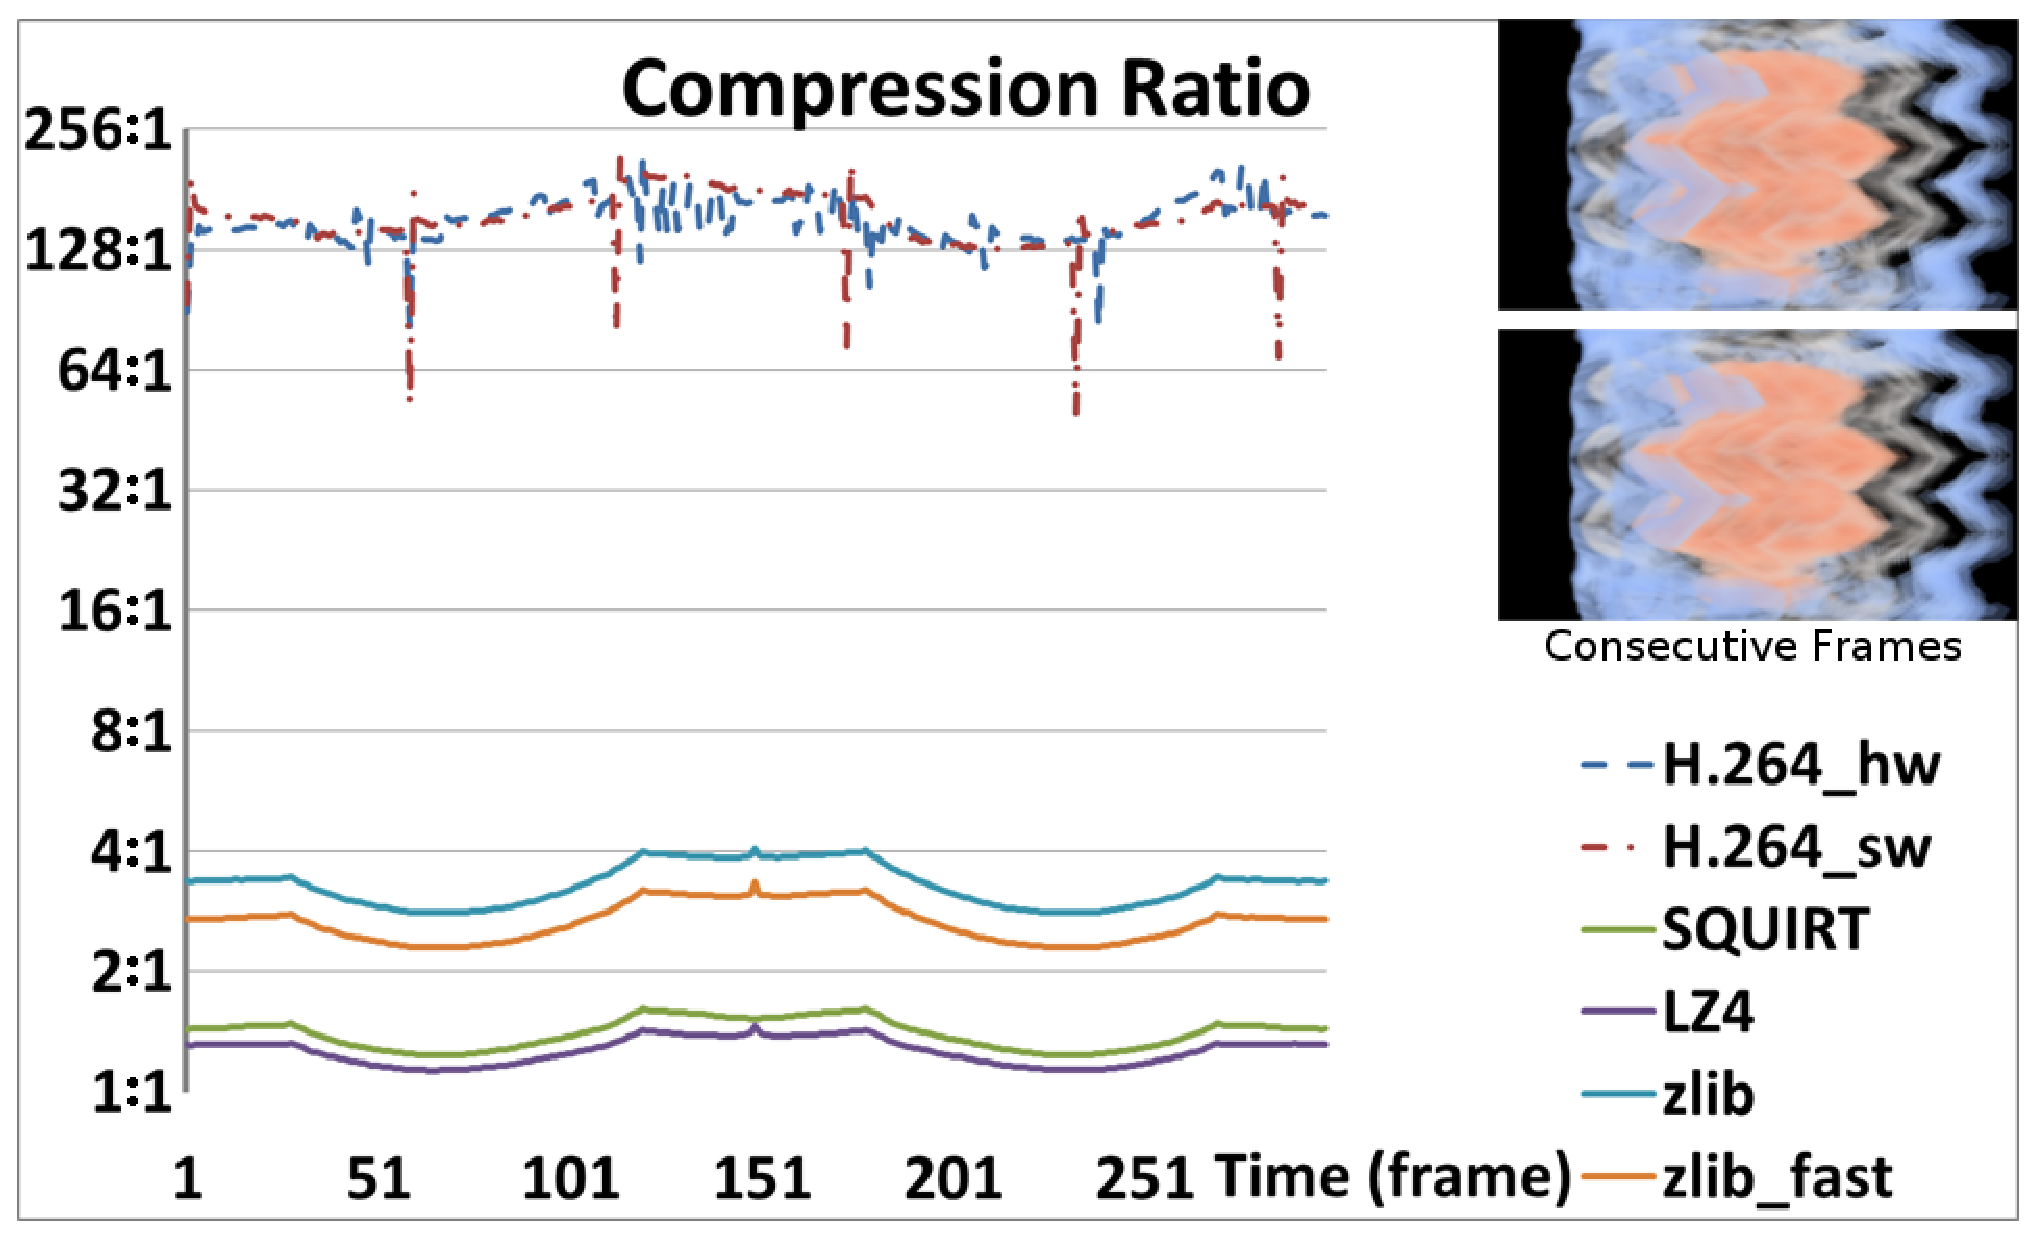
\includegraphics[width=2.0in]{compressRatio.eps}
  \caption{Real-time compression ratio during 100-frame visualization of rotating wavelet data at 1080P}
\end{figure}

% discuss encoding/decoding time --> framerate / latency 
\begin{figure}[htb]
  \label{figure:time}
  \centering
  \includegraphics[width=1.8in]{encodingTime.eps}
  \includegraphics[width=1.8in]{decodingTime.eps}
  \caption{Average compress and decompress time per frame in milliseconds. Image resolution is 1920x1080. For NvPipe we stack the time for image conversion and encoding/decoding time}
\end{figure}

\subsection{Conclusion}

NvPipe demonstrate enormous advantage on compression ratio over other image compressors at no extra computational time. It could greatly reduce the communication latency and increase the achievable framerate of remote visualization system with limited bandwidth.

Although for scientific visualization, the compression process produces no perceivable errors. In future research it will definitely be interesting to investigate the lossless HEVC codec available with NVIDIA codec 7.0 API.

%\acknowledgements{
%NVIDIA standard acknowledgement for funding?
%}

\bibliographystyle{abbrv}
%%use following if all content of bibtex file should be shown
\nocite{*}
\bibliography{template}
\end{document}
